
\chapter{模板生成和内容提取}
\label{chap:template}
\section{模板定义}
我们在第~\ref{sec:htmltemplateintro}节中介绍了模板直观上的定义:不同网页公共的部
分。我们期望从目前得到的大量的由同一模板生成的网页集合中,找出那些反复出现的网页
结构,将其作为这些网页的模板。

这里我们将首先形式化定义模板的组成。模板的基本元素是基本节点(Base Node),每
个节点有两种形式:
\begin{enumerate}
\item 单个不重复的HTML标签,即$<tag>$
\item 由一个或多个HTML标签组成的序列,这些序列可以出现一次或多
  次,即$(\sum_{i=1}^N<tag_i>)+$,其中$N \ge 1$
\end{enumerate}
这里的$+$表示可以出现一次或者多次,沿用的是正则表达式的习惯。可以看到基本节点与经
过预处理去除重复记录后的序列节点是对应的。第一种基本节点对应没有合并的序列节点,
第二种基本节点对应着多个重复记录合并后的序列节点,由于是一个“记录”,因此可以由
一个或多个标签组成,并且可以重复出现。

基本节点的序列可以组成必选节点(Essential Node)或可选节点(Optional Node)。必选
节点对应着由基本节点组成的一个序列,若基本节点用$tn_i$表示,则必选节点$EN$可以表
示为:
\[
EN=tn_1tn_2...tn_n
\]
可选节点$ON$则同时对应多个序列,每个序列由不同的基本节点组成,同时每个序列还对应
着一个出现概率$p$,即:
\[
ON=(tn_{11}tn_{12}...tn_{1n_1},p_1)|(tn_{21}tn_{22}...tn_{2n_2},p_2)|...|(tn_{k1}tn_{k2}...tn_{kn_k},p_k)
\]
这里$|$表示“或”的关系。

我们规定模板中必选节点和可选节点必须间隔出现,一个模板(Template)$Tp$可以定义为
这样一个序列:
\[
Tp=[ON_0]EN_1ON_1EN_2ON_2......EN_n[ON_n]
\]
其中第一个可选节点$ON_0$和最后一个可选节点$ON_n$都不是必需的。
\section{模板生成}
\label{sec:templategen}
通过聚类,我们已经得到了一些由同一种模板生成的网页集合,接下来我们将对每个聚类单
独进行处理,生成对应的模板。设当前我们处理的聚类为$c$,聚类的中心点
是$p_{center}$,类中的点$p_i$对应的序列为$s_i$。

根据定义,我们需要生成一个必选节点和可选节点交替出现的序列。我们的方法是:先生成
全部的必选节点,然后在中间插入可选节点。

必选节点,顾名思义就是在该模板生成的网页中,必选节点中包含的所有基本节点都应该出
现。因此,我们需要求出在$c$中每个序列都出现的那些标签序列$s_{common}$。做法是从聚
类的中心点$p_{center}$出发,将其对应的序列$s_{center}$作为$s_{common}$的初始值,
依次与$c$中的每一个序列求一次最长公共子序列$lcs$,并将$s_{common}$的值更新
为$lcs$。迭代结束时得到的标签序列就是组成必选节点的所有的基本节点。算法如伪代
码~\ref{template:algo:common}所示。
\begin{algorithm}
  \caption{得到组成必选节点的所有基本节点}
  \label{template:algo:common}
  \begin{algorithmic}[1]
    \Require 输入聚类$c$
    \Ensure 得到$c$中所有文档共有的序列$s_{common}$
    \Function{findCommonSequence}{$c$}
    \State $//$初始化为中心点所对应的序列
    \State $s_{common} := c.s_{center}$
    \State $//$依次求最长公共子序列
    \For{$s_i \gets c.sequences$}
    \State $lcs := getLCS(s_i, s_{common})$
    \State $s_{common} := lcs$
    \EndFor
    \State \Return $s_{common}$
    \EndFunction
  \end{algorithmic}
\end{algorithm}

以上得到的序列只是所有网页结构的公共部分,每个由这个模板生成的网页都应该有这个结
构,然而这并不是模板的全部组成。我们考虑到很多后台模板生成网页时可能会使用一些条
件分支控制结构,如if,因此仅仅由上述的序列组成模板是不够的。仍然以Django为例,有
些网页的标题可能有副标题,而有些可能没有,在Django框架的模板语言中,可以写成
如\reffig{template:fig:django-if}所示的模板片段。根据这个模板的定
义,\texttt{<h2>}标签并不一定会在全部的由该模板生成的网页中出现,但我们在模板生成
的时候必须考虑到这种情况,否则有些内容比如\texttt{<h2>}对应的“副标题”就没法正确
提取了。为此,我们引入了可选节点。因为实际的模板中可能会有多种不同的条件分支,所
以每个可选节点对应多个不同的基本节点的序列,这些序列不一定在每个网页中都出现,每
个序列都对应着一定的出现概率。

\begin{figure}
  \centering
  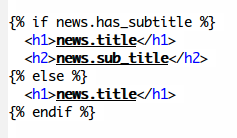
\includegraphics[width=0.3\textwidth]{template05/django-if}
  \caption{Django带条件判断的模板}
  \label{template:fig:django-if}
\end{figure}

以下我们举个简化的例子来说明构造可选节点的基本思想。设有3个序列,分别为:
\begin{eqnarray*}
s_1&=&aorzbcdlxe\\
s_2&=&athubeatcdlxe\\
s_3&=&athubeatcdpkue
\end{eqnarray*}

首先,根据算法~\ref{template:algo:common},得到$s_{common}$为$abcde$。然后,我们
将每个序列同$s_{common}$进行对齐,得到
\[
\begin{matrix}
s_1      &:&\mathbf{a}&orz&\mathbf{b}&   &\mathbf{cd}&lx&\mathbf{e}\\
s_2      &:&\mathbf{a}&thu&\mathbf{b}&eat&\mathbf{cd}&lx&\mathbf{e}\\
s_3      &:&\mathbf{a}&thu&\mathbf{b}&eat&\mathbf{cd}&pku&\mathbf{e}\\
s_{common}&:&\mathbf{a}&   &\mathbf{b}&   &\mathbf{cd}&   &\mathbf{e}
\end{matrix}
\]

我们利用每个序列同$s_{common}$对齐的结果,对每个序列进行分割,我们
用$s_i[t_1,t_2]$表示序列$s_i$在对齐的标签$t_1,t_2$之间的部分,如$s_3[a,b]$表示序
列$thu$。对于每一个区间$[t_1,t_2]$,如果文档集合中的某些序列有未对齐的部分,
即$\exists s_i,|s_i[t_1,t_2]| > 0$,我们将对应生成一个可选节
点$ON_{t_1,t_2}$,这个可选节点对应于这个区间中所有未对齐的子序列。在我们的例
子中,我们生成以下三个可选节点:
\begin{eqnarray*}
  ON_{a,b}&=&thu,2/3~|~orz,1/3\\
  ON_{b,c}&=&eat,2/3\\
  ON_{d,e}&=&lx,2/3~|~pku,1/3
\end{eqnarray*}

对齐的部分则对应生成必选节点,分别为:$a,b,cd,e$。将这些必选节点和可选节点间隔地
依次组成一个序列,这3个序列对应的模板就生成好了。

由以上的例子,我们可以得到模板生成子模块的整体流程图
如\reffig{template:fig:subsystem}所示,
\begin{figure}
  \centering
  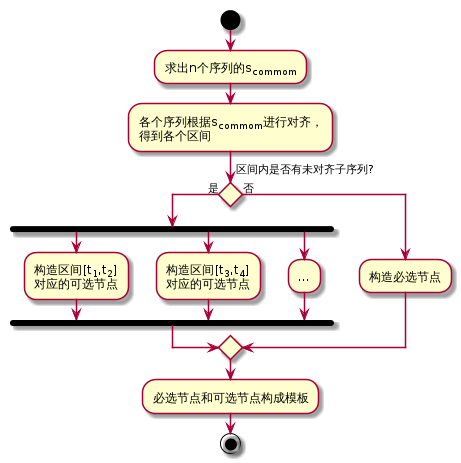
\includegraphics[width=0.7\textwidth]{template05/subsystem}
  \caption{模板生成子模块整体流程图}
  \label{template:fig:subsystem}
\end{figure}

然而,实际的情况却要比上面的例子更复杂一些。对于实际的网页文档集合,区
间$[t_1,t_2]$中未对齐的那些标签子序列,有些可能差异很大,有些则可能非常相近,但不
完全一样。因此,我们需要将\reffig{template:fig:subsystem}中构造可选节点的过程进一
步细化:先将这些子序列中差异较大的几种模式分开,然后针对每个分好的类别提取其中共
有的部分,用于构造可选节点。

根据以上的叙述,我们发现,构造可选节点的这个子问题和我们的系统要解决的问题有很大
的相似性,都可以简单描述为:存在一个序列集合,里面的元素由几种不同的模式生成,需
要先将这些元素分成几种类别,然后针对每个类别去提取公共的部分,即“模板”。对于构
造可选节点这个子问题而言,这里的“模板”指的是在那些子序列的聚类中反复出现的模式,
和我们要最终要提取的网页模板有很大的相似性。为了叙述简便,我们不妨称之为“子模
板”。

提取这些子模板的过程和系统的整体框架极其类似。对于每个存在未对齐子序列的区
间$[t_1,t_2]$:
\begin{enumerate}
\item 区间内所有未对齐的序列组成一个新的序列集合$set_{s'}$。
\item 把集合$set_{s'}$放入之前的聚类模块中,根据算
  法~\ref{cluster:algo:clustering}得到聚类的结果$clusters$。
\item 针对$clusters$中的每个聚类$c$,使用算法~\ref{template:algo:common}得到它
  的“子模板”,并根据聚类$c$的大小和原始文档集合之间的大小,计算这个“子模板”的
  出现概率$p$。
\end{enumerate}

这样,区间$[t_1,t_2]$得到一个由多个子模板和其对应的出现概率组成的序列,这个序列就
组成了区间$[t_1,t_2]$所对应的的可选节点。必选节点则根据对齐结果生成,主要是将一些
连续的中间没有未对齐序列的基本节点合并成一个必选节点,如上面的例子中,我们
将$c,d$两个基本节点合并成了一个必选节点。这些必选节点和可选节点组成的序列也就构成
了我们要处理的这个聚类的模板了。
\begin{figure}
  \centering
  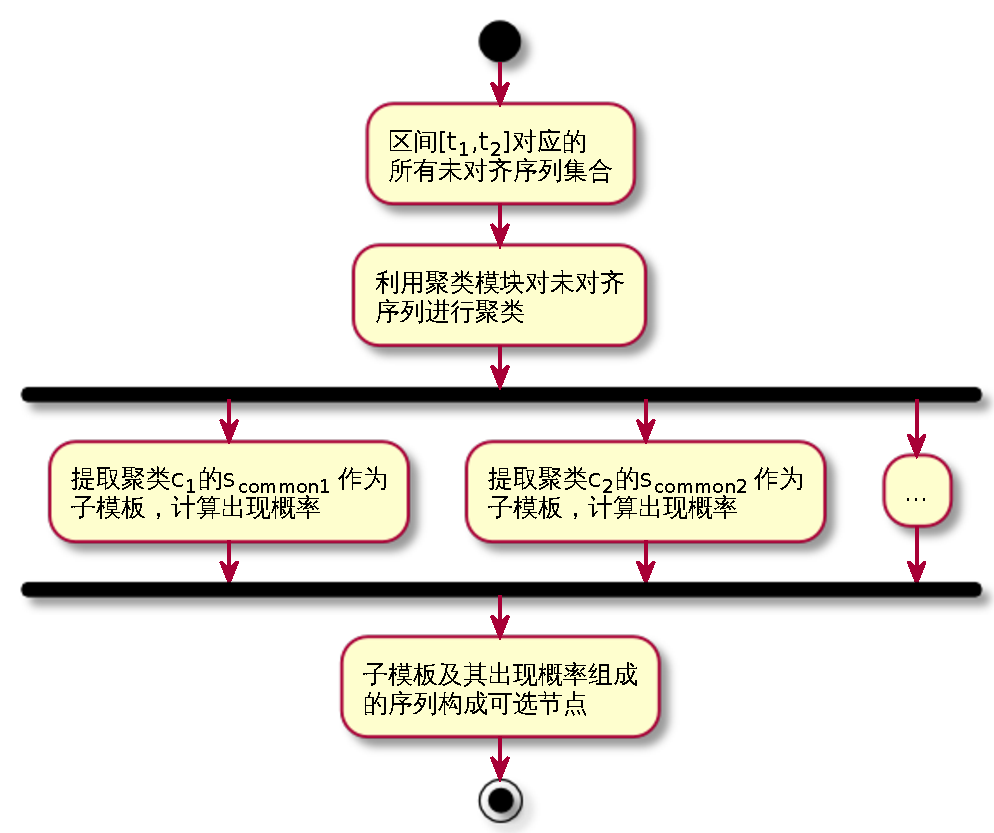
\includegraphics[width=0.7\textwidth]{template05/subtemplate}
  \caption{细化的构造可选节点的流程图}
  \label{template:fig:subtemplate}
\end{figure}

细化以后的构造可选节点的流程如\reffig{template:fig:subtemplate}所示。

最后,观察到从\reffig{template:fig:subsystem}中构造各个可选节点的过程是并行的,因
此为了加快模板的计算速度,我们在这里再次使用了Actor模型并行地计算每个可选节点。

我们对每一个聚类都生成一个模板,这些模板将作为我们系统训练的输出,用于提取新的网
页中的内容。
\section{内容提取}
\label{sec:extraction}
这个子模块中,我们将利用聚类模块得到的聚类和前一个子模块生成好的模板,对新输入的
网页进行内容的提取。

作为内容提取的第一步,我们需要先针对每个模板做一些简单的人工标注。由于整个模板生
成的过程是无监督的,中间也没有考虑模板对应部分的语义信息,因此,在自动生成好模板
后,还需要通过人工指定语义的办法使得系统能够判断哪部分的内容才是我们真正所关心的。
比如当我们生成好了一类新闻网页的模板后,我们可以手工在模板的对应部分标
上“标题”,“正文”和“评论”等,这样后续的内容提取部分就能自动将这些内容提取出
来。

第二步需要先将新输入的网页经过预处理模块进行处理,包括去掉无用标签、合并重复记录
等等,得到一个新的输入序列,计算这个序列和我们得到的每个聚类中心的距离,得到这些
距离的最小值。如果这个最小值大于聚类时设置的阈值,则认为出现了一个新模板生成的网
页,将其暂时存储,不进行处理。否则,我们选择与之距离最近的聚类对应的生成好的模板
作为这个新的网页内容提取的模板。

第三步,与模板生成模块类似,我们首先用模板中的必选节点对齐序列,然后对于每个存在
未对齐序列的区间,我们找到对应的可选节点,优先使用出现概率高的序列进行对齐。把所
有的有未对齐序列的区间中的序列进行了对齐之后,那些原序列中尚未匹配的节点就是网页
中动态生成的部分,也就是我们提取出来的内容。这时我们根据之前的人工标注,筛选出我
们关心的部分,将其存为XML格式,作为输出。

内容提取子模块的整体框架如\reffig{template:fig:extractor}所示。
\begin{figure}
  \centering
  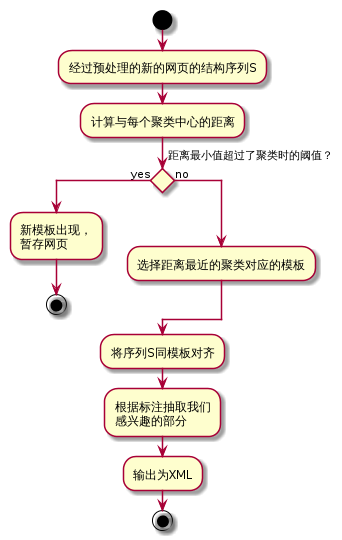
\includegraphics[width=0.5\textwidth]{template05/extractor}
  \caption{内容提取子模块的整体框架}
  \label{template:fig:extractor}
\end{figure}

这里还需要补充两点:第一,由于之前合并了重复记录,因此在提取内容的时候需要进行复
原,将其对应到原网页的多条内容上;第二,对于不属于任何类别的新的模板生成的网页,
我们将其暂存,当其数量到达一定值的时候,我们将用这些网页进行训练,得到新的模板,
加入到现有的系统中,从而实现了新模板的自动识别和生成功能。

\section{本章总结}
\label{sec:summarytemplate}
在这一章中,我们介绍了模板生成和内容提取模块的实现。为了讨论方便,我们首先形式化
地定义了模板,然后我们介绍了如何对每个聚类生成对应的模板,重点在于如何正确构造模
板中的可选节点。最后我们介绍了内容提取模块的具体实现流程。

至此,我们系统的各个模块的具体实现都已经介绍完了。

%%% Local Variables: 
%%% mode: latex
%%% TeX-master: "../main"
%%% End: 
